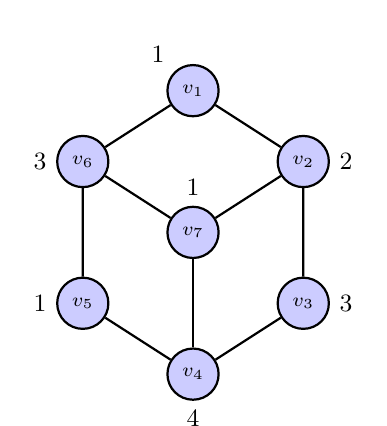
\begin{tikzpicture}[
  baseline=0pt,
  scale=1,
  vnode/.style={circle, draw=black, fill=blue!20, thick, inner sep=0pt, minimum size=6.5mm},
  edge/.style={thick, draw=black},
  clabel/.style={font=\small, color=black}
]
  \useasboundingbox (-2.1,-2.3) rectangle (2.1,2.4);

  \begin{scope}[yshift=-0.2cm]
    % 7 Vértices
    \node[vnode, label={[clabel]above left:$1$}] (v1) at (0.0, 1.8) {$\scriptstyle v_1$};
    \node[vnode, label={[clabel]right:$2$}]        (v2) at (1.4, 0.9) {$\scriptstyle v_2$};
    \node[vnode, label={[clabel]right:$3$}]        (v3) at (1.4, -0.9) {$\scriptstyle v_3$};
    \node[vnode, label={[clabel]below:$4$}]        (v4) at (0.0, -1.8) {$\scriptstyle v_4$};
    \node[vnode, label={[clabel]left:$1$}]         (v5) at (-1.4, -0.9) {$\scriptstyle v_5$};
    \node[vnode, label={[clabel]left:$3$}]         (v6) at (-1.4, 0.9) {$\scriptstyle v_6$};
    \node[vnode, label={[clabel]above:$1$}]        (v7) at (0.0, 0.0) {$\scriptstyle v_7$};

    % Aristas
    \draw[edge] (v1) -- (v2) -- (v3) -- (v4) -- (v5) -- (v6) -- (v1);
    \draw[edge] (v7) -- (v2);
    \draw[edge] (v7) -- (v6);
    \draw[edge] (v7) -- (v4);
  \end{scope}
\end{tikzpicture}
